\section{Experimental setup and conduction}
\label{sec:experimental_setup_and_conduction}

This section introduces the experimental setup in \autoref{sec:setup} and the conduction in \autoref{sec:conduction}.
\subsection{Experimental setup}
\label{sec:setup}
This experiment uses the Alibava EASy detector system. A schematic setup is shown in \autoref{fig:setup}.\begin{figure}[h]
\centering
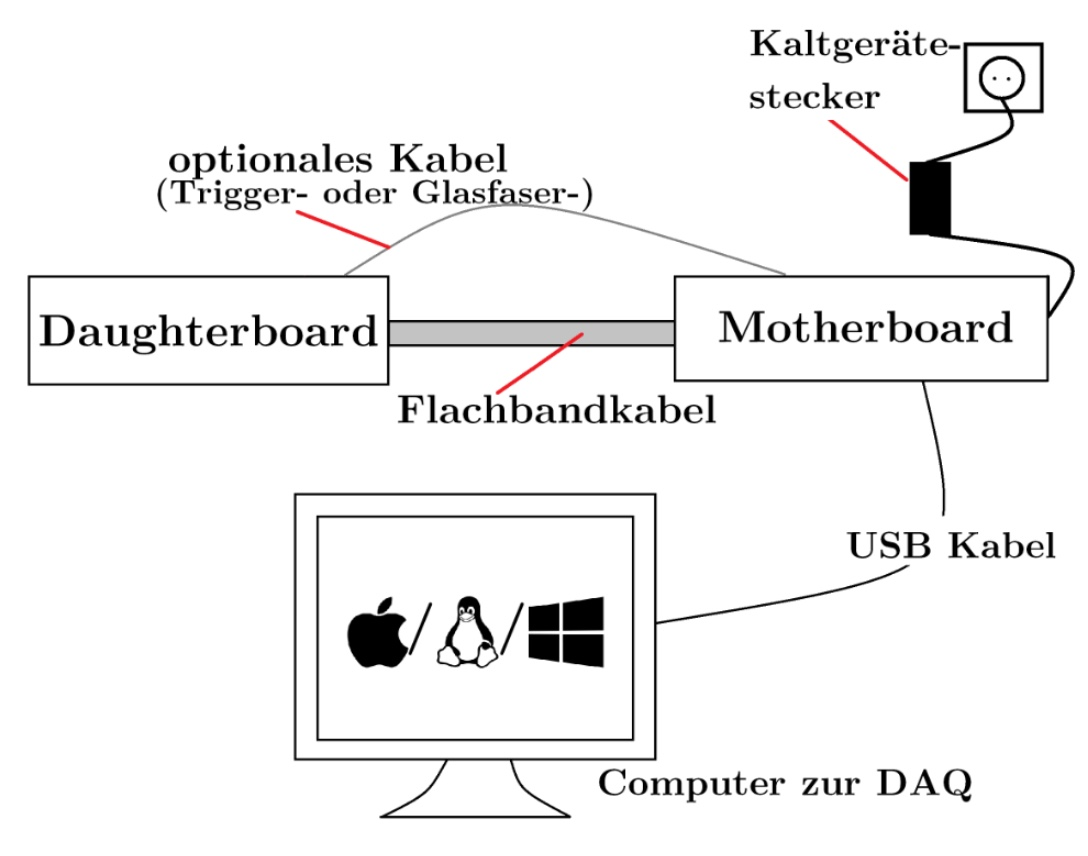
\includegraphics[width=0.8\textwidth]{content/Figures/setup.jpeg}
\caption{Schematic setup of the Alibava EASy detector system \cite{Vorlage}.}
\label{fig:setup}
\end{figure}
The system consists of three main elements: the detector unit, the control unit and a computer running the Alibava software. The detector unit contains the silicon semiconductor sensor and the front-end readout electronics. These components are located on the daughterboard, which carries the BEETLE readout chip. The BEETLE chip amplifies the charge signals induced in the sensor and converts them into voltage signals.

The motherboard in the control unit handles the timing, trigger processing and communication with the computer. It receives an incoming trigger signal, which defines when an event should be read out. After a chosen delay, the control unit digitizes the voltage signal into ADC counts. This delay is adjusted such that the signal maximum is measured.

The current-voltage measurement makes sure that the sensor is fully depleted. This measurement is introduced in \autoref{sec:conduction}. The sensor has a $\SI{300}{\micro\meter}$ thick n-doped silicon layer, which is covered with a metallization. On top there are $\num{128}$ p-doped strips, which are separated and used for localization.

Furthermore, a laser with a wavelength of $\SI{980}{\nano\meter}$ can be attached to the detector unit and adjusted with screws for the laser measurement, which is also introduced in \autoref{sec:conduction}.

\subsection{Conduction}
\label{sec:conduction}
At first there is a current-voltage measurement. In this case the voltage is set at the control unit from $\SI{0}{\volt}$ to $\SI{200}{\volt}$ with the stepsize of $\SI{10}{\volt}$. The current is plotted against the voltage. The voltage is set to $\SI{90}{\volt}$, where the sensor is fully depleted.\\\\
Then a Pedestals run is performed for $\num{1000}$ events. This calculates the noise from the background with the mean ADC value without a signal, which is called pedestal. This measurement is used to reduce the fluctuations of the signal.\\\\
The next step is the calibration measurement. At first there is a delay measurement performed, to calibrate the system to the delay with the maximum of signal. The delay of $\SI{64}{\nano\second}$ is set. Then the calibration runs with different strips are measured. Therefore the strip numbers are set from $\num{28}$ to $\num{124}$ with the stepsize of $\num{24}$. There is also a measurement where the voltage is set to $\SI{0}{\volt}$ for comparing this result with a fully depleted sensor.\\\\
In the next measurement the Laser is integrated and focused with a vertical srew such that the signal becomes the maximum. Then the Laserposition is set from $\SI{10}{\micro\meter}$ to $\SI{350}{\micro\meter}$ with the stepsize of $\SI{10}{\micro\meter}$ to analyze the strip structure.\\\\
For the last measurement the Laserposition is set to $\SI{230}{\micro\meter}$ and the voltage from $\SI{0}{\volt}$ to $\SI{200}{\volt}$ with the stepsize of $\SI{10}{\volt}$ and recorded with a dataset of $\num{1000}$ events. This is used to analyze the determine the efficiency of the charge collection in \autoref{sec:Analysis}.
